\section{Methodology Validation}

In the last chapter, the survival probability $S(\tau)$ and the mean
first-passage time has been calculated by solving the heat equation
and approximated by the numerical methods. Lattice Random Walks (LRWs)
and Pearson's Random Walks (PRWs) are implemented in the annulus
image, as shown in Figure~\ref{fig:annulus}, in Python. This section
aims to validate the research methodology by comparing the estimated
survival functions $S(t)$ of the numerical data with the analytical
solutions $S(\tau)$ where $t$ is the number of steps taken by the
particles in the fixed-time step Monte Carlo simulations and $\tau$
denotes the unitless time.


\subsection{Statistical Fluctuation Analysis}

Fixed-time step Monte Carlo simulations, LRWs and PRWs, are the
nondeterministic numerical representations of the original statistical
problem defined in the continuous-time and continuous-space with
numerous inputs and discrete-time trajectories. In the simulations,
the initial positions of the enormous number of particles and their
moving directions at each time step are determined by the randomly
uniform sampling. Thus, it is inevitable to appear the statistical
fluctuations, also called variance, defined as a measure of the
discrepancies between the estimate and the true solution. The
brute-force way to reduce the statistical fluctuations is to increase
the sample size.


The first kind of error stems from the sampling. As shown in
Figure~\ref{fig:annulus_32_particles} and
Figure~\ref{fig:annulus_256_particles}, the larger sample size in the
simulations, the estimated survival functions will be more
precise. LRWs are used to mimic the continuous-time and
continuous-space diffusion process by generating the discrete random
trajectories in the discrete time, which results in the
time-discretization and space-discretization errors. Although PRWs is
a model defined in continuous-time and continuous-space, the random
paths demand much longer time simulation as shown in
Figure~\ref{fig:annulus_finer_steps}.

\begin{figure}
  \begin{subfigure}{0.9\textwidth}
    \centering
    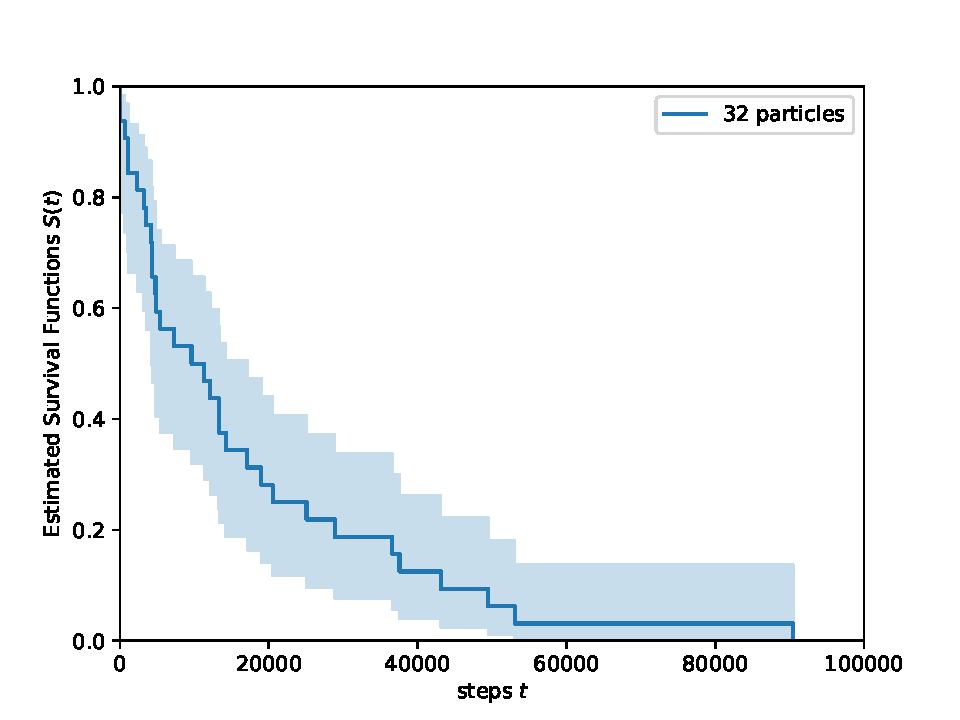
\includegraphics[width=0.8\textwidth]{sampling_32}
    \caption{Survival curve for the LRWs with $32$ particles.\label{fig:annulus_32_particles}}
  \end{subfigure}
  \begin{subfigure}{0.9\textwidth}
    \centering
    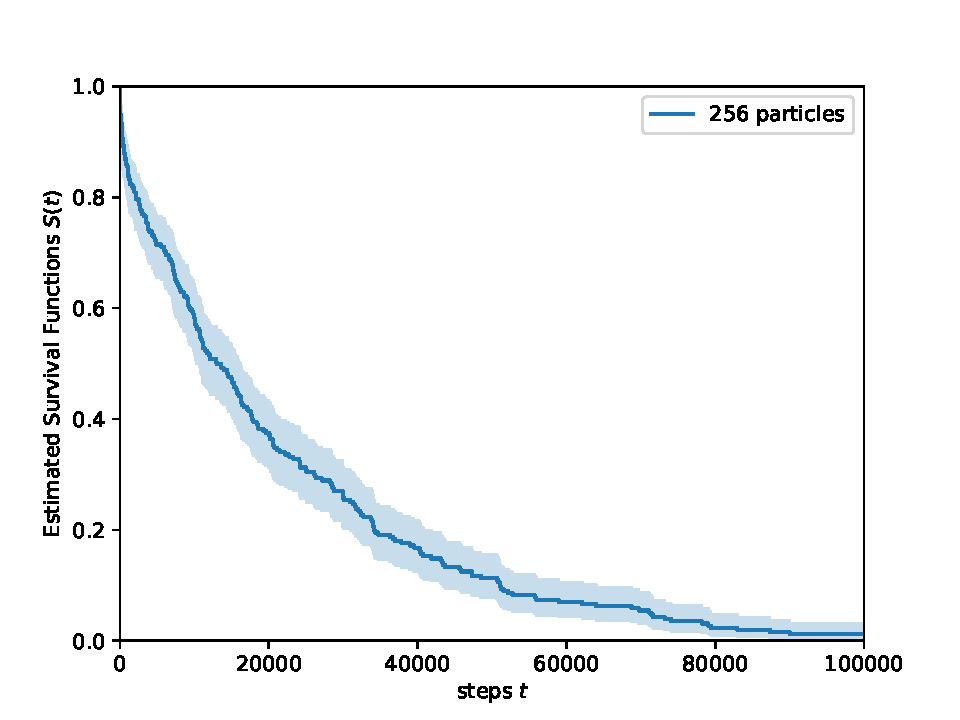
\includegraphics[width=0.8\textwidth]{sampling_256}
    \caption{Survival curve for the LRWs with $256$ particles. \label{fig:annulus_256_particles}}
  \end{subfigure}
  \caption{Estimated survival curves and 95\% confidence intervals for
    Monte Carlo simulations of partical diffusion on an annulus. As
    the number of particles increasing, the uncertainty of the LRWs
    simulation are lower since the confidence band of the estimated
    survival function becomes narrower.\label{fig:lrw_prw_annulus}}
\end{figure}



\begin{figure}
  \centering
  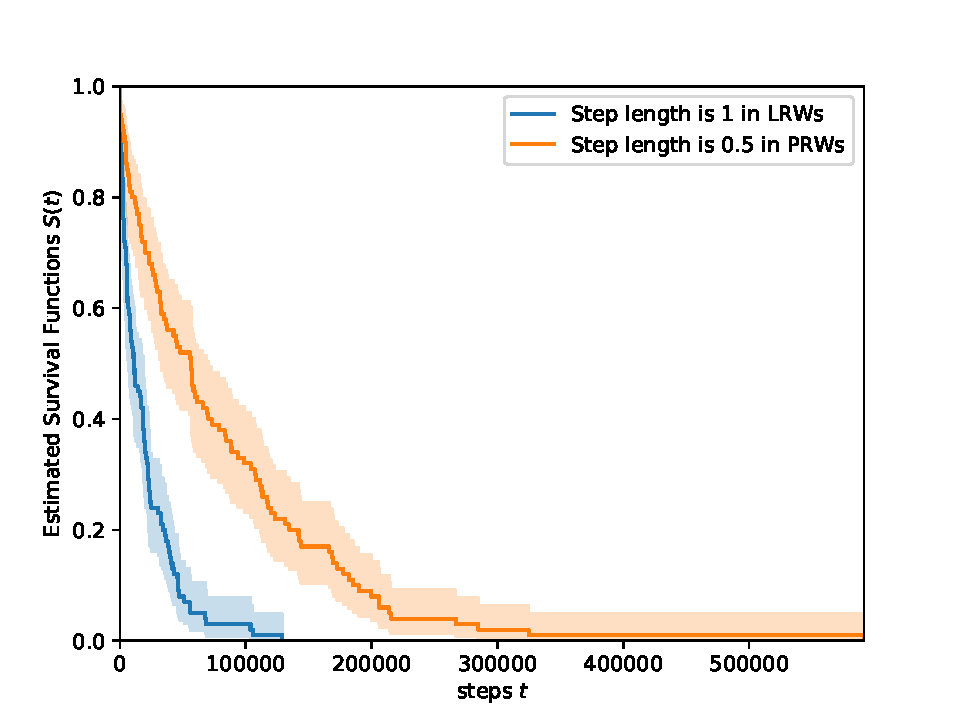
\includegraphics[width=0.8\textwidth]{discretization}
  \caption{When run LRWs and PRWs in the annulus with $100$ particles,
    the finer discretization step results in the longer simulation
    time.\label{fig:annulus_finer_steps}}
\end{figure}
